\documentclass{article}
\usepackage{amsmath, tikz, xcolor, enumitem}
\usetikzlibrary{arrows.meta, calc}
\everymath{\displaystyle}
\pagestyle{empty}
\raggedright
\usepackage[margin = 0.5in]{geometry}
\begin{document}

Name \makebox[3in]{\hrulefill} \hfill Honors PreCalc P-Set

\subsubsection*{Polar Coordinates \hfill \makebox[0.35in]{\hrulefill} / 10}

Plot each on the grid and label your points.    \newline\\
\begin{minipage}{0.6\textwidth}
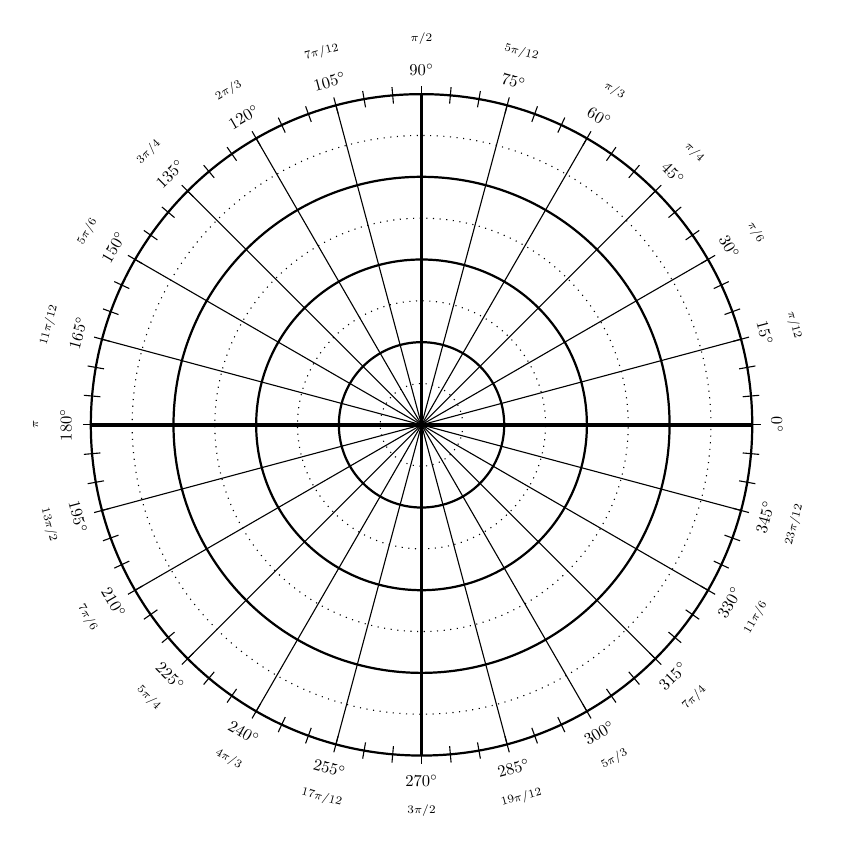
\begin{tikzpicture}[scale = 0.7, every node/.style={scale=0.6}]
    % Origin Point
    \coordinate (O) (0,0);
    % Circles
    \foreach \r in {1.5,3,...,6}
    {
        \draw[thick] (O) circle (\r cm);
    }
    
    % \foreach \r in {1.5,3,...7.5}
    % {
    %     \node at (\r, 0) [anchor=north] {\r/};
    % }
    
    \foreach \r in {0.75, 2.25,...,5.25}
    {
        \draw[dotted] (O) circle (\r cm);
    }
    
    % \node at (1.5, 0) [anchor = north west] {1};
    % \node at (3, 0) [anchor = north west] {2};
    % \node at (4.5, 0) [anchor = north west] {3};
    % \node at (6, 0) [anchor = north west] {4};
    % \node at (7.5,0) [anchor = north west] {5};
    % \foreach \r in {1.5,3,...,9}
    % {
    %     \node at (\r, 0) {\r/1.5};
    % }
    % Radial Lines
    \foreach \l in {0,15,...,360}
    {
        \draw (O) -- ++(\l:6cm);
    }
    % Thicker Radial Lines at 90 degree increments
    \foreach \l in {0,90,...,360}
    {
        \draw[very thick] (O) -- ++(\l:6cm);
    }
    % Minor Tick marks on outer circle
    \foreach \t in {0,5,...,360}
    {
        \draw (O) ++ (\t:5.85cm) -- ++(\t:0.3cm);
    }
    % Now for the fun part, the text
    % Degrees
    \node[draw=none, rotate= -90 ] at ( 0 :6.45cm) {$ 0 ^\circ$};
    \node[draw=none, rotate= -75 ] at ( 15 :6.45cm) {$ 15 ^\circ$};
    \node[draw=none, rotate= -60 ] at ( 30 :6.45cm) {$ 30 ^\circ$};
    \node[draw=none, rotate= -45 ] at ( 45 :6.45cm) {$ 45 ^\circ$};
    \node[draw=none, rotate= -30 ] at ( 60 :6.45cm) {$ 60 ^\circ$};
    \node[draw=none, rotate= -15 ] at ( 75 :6.45cm) {$ 75 ^\circ$};
    \node[draw=none, rotate= 0 ] at ( 90 :6.45cm) {$ 90 ^\circ$};
    \node[draw=none, rotate= 15 ] at ( 105 :6.45cm) {$ 105 ^\circ$};
    \node[draw=none, rotate= 30 ] at ( 120 :6.45cm) {$ 120 ^\circ$};
    \node[draw=none, rotate= 45 ] at ( 135 :6.45cm) {$ 135 ^\circ$};
    \node[draw=none, rotate= 60 ] at ( 150 :6.45cm) {$ 150 ^\circ$};
    \node[draw=none, rotate= 75 ] at ( 165 :6.45cm) {$ 165 ^\circ$};
    \node[draw=none, rotate= 90 ] at ( 180 :6.45cm) {$ 180 ^\circ$};
    \node[draw=none, rotate= 285 ] at ( 195 :6.45cm) {$ 195 ^\circ$};
    \node[draw=none, rotate= 300 ] at ( 210 :6.45cm) {$ 210 ^\circ$};
    \node[draw=none, rotate= 315 ] at ( 225 :6.45cm) {$ 225 ^\circ$};
    \node[draw=none, rotate= 330 ] at ( 240 :6.45cm) {$ 240 ^\circ$};
    \node[draw=none, rotate= 345 ] at ( 255 :6.45cm) {$ 255 ^\circ$};
    \node[draw=none, rotate= 360 ] at ( 270 :6.45cm) {$ 270 ^\circ$};
    \node[draw=none, rotate= 375 ] at ( 285 :6.45cm) {$ 285 ^\circ$};
    \node[draw=none, rotate= 390 ] at ( 300 :6.45cm) {$ 300 ^\circ$};
    \node[draw=none, rotate= 405 ] at ( 315 :6.45cm) {$ 315 ^\circ$};
    \node[draw=none, rotate= 420 ] at ( 330 :6.45cm) {$ 330 ^\circ$};
    \node[draw=none, rotate= 435 ] at ( 345 :6.45cm) {$ 345 ^\circ$};
    % Radians

    \node[draw=none, rotate= -90 ] at ( 0 :7cm) {$  $};
    \node[draw=none, rotate= -75 ] at ( 15 :7cm) {\scriptsize$ \pi/12 $};
    \node[draw=none, rotate= -60 ] at ( 30 :7cm) {\scriptsize$ \pi/6 $};
    \node[draw=none, rotate= -45 ] at ( 45 :7cm) {\scriptsize$ \pi/4 $};
    \node[draw=none, rotate= -30 ] at ( 60 :7cm) {\scriptsize$ \pi/3 $};
    \node[draw=none, rotate= -15 ] at ( 75 :7cm) {\scriptsize$ 5\pi/12 $};
    \node[draw=none, rotate= 0 ] at ( 90 :7cm) {\scriptsize$ \pi/2 $};
    \node[draw=none, rotate= 15 ] at ( 105 :7cm) {\scriptsize$ 7\pi/12 $};
    \node[draw=none, rotate= 30 ] at ( 120 :7cm) {\scriptsize$ 2\pi/3 $};
    \node[draw=none, rotate= 45 ] at ( 135 :7cm) {\scriptsize$ 3\pi/4 $};
    \node[draw=none, rotate= 60 ] at ( 150 :7cm) {\scriptsize$ 5\pi/6 $};
    \node[draw=none, rotate= 75 ] at ( 165 :7cm) {\scriptsize$ 11\pi/12 $};
    \node[draw=none, rotate= 90 ] at ( 180 :7cm) {\scriptsize$ \pi $};
    \node[draw=none, rotate= 285 ] at ( 195 :7cm) {\scriptsize$ 13\pi/2 $};
    \node[draw=none, rotate= 300 ] at ( 210 :7cm) {\scriptsize$ 7\pi/6 $};
    \node[draw=none, rotate= 315 ] at ( 225 :7cm) {\scriptsize$ 5\pi/4 $};
    \node[draw=none, rotate= 330 ] at ( 240 :7cm) {\scriptsize$ 4\pi/3 $};
    \node[draw=none, rotate= 345 ] at ( 255 :7cm) {\scriptsize$ 17\pi/12 $};
    \node[draw=none, rotate= 360 ] at ( 270 :7cm) {\scriptsize$ 3\pi/2 $};
    \node[draw=none, rotate= 375 ] at ( 285 :7cm) {\scriptsize$ 19\pi/12 $};
    \node[draw=none, rotate= 390 ] at ( 300 :7cm) {\scriptsize$ 5\pi/3 $};
    \node[draw=none, rotate= 405 ] at ( 315 :7cm) {\scriptsize$ 7\pi/4 $};
    \node[draw=none, rotate= 420 ] at ( 330 :7cm) {\scriptsize$ 11\pi/6 $};
    \node[draw=none, rotate= 435 ] at ( 345 :7cm) {\scriptsize$ 23\pi/12 $};
\end{tikzpicture} 
\end{minipage}
\begin{minipage}{0.2\textwidth}
1. \quad $A\left(2, \frac{3\pi}{4}\right)$ \\[0.5cm]
2. \quad $B\left(-3.5, -75^\circ \right)$  \\[0.5cm]
3. \quad $C\left(1, -\frac{7\pi}{6}\right)$ \\[0.5cm]
4. \quad $D\left(-3, 240^\circ\right)$
\end{minipage}
\newline\\
Convert each of the following to rectangular form. Use exact values when applicable.
\begin{flalign*}
5. \quad    &   \left(5, \, \frac{7\pi}{4}\right)           &
6. \quad    &   \left(11, \, -\frac{7\pi}{6}\right)         &
7. \quad    &   \left(-4, \, \frac{5\pi}{6}\right)         &
8. \quad    &   \left(9, \, \frac{7\pi}{2}\right)          &&\\[1in]
\end{flalign*}

Convert each of the following to polar form. Use exact values when applicable.
\begin{flalign*}
9. \quad    &   \left( -\sqrt{2}, \, \sqrt{2} \right) &
10. \quad    &   \left( -4, \, -4\sqrt{3} \right)      &&\\[1in]
11. \quad    &   \left( \frac{\sqrt{3}}{4}, \, -\frac{1}{4} \right)    &
12. \quad    &   \left( -\sqrt{5}, \, -\sqrt{5} \right)    &&\\
\end{flalign*}


\newpage

Convert each rectangular equation to a polar one.
	\begin{flalign*}
	13. \quad	&	5x + 7y = 10		&
	14. \quad	&	y = 2x - 1			&
	15. \quad	&	x - y = 9		    &&\\[2.5in]
	\end{flalign*}
	
Convert each polar equation to a rectangular one.
	\begin{flalign*}
	16. \quad	&	r = 4 \cos \theta	&
	17. \quad	&	r = 2 \sin \theta	&
	18. \quad	&	r = \dfrac{3}{\sin \theta}	&&\\[2.75in]
	19. \quad	&	r = 3 \sec \theta	&
	20. \quad	&	r = -5				&
	21. \quad	&	\theta = \frac{\pi}{4}	&&\\
	\end{flalign*}




% \fbox{\emph{Level 2}}
% \newline\\


% Find the intersection(s) of the two functions.
% \begin{flalign*}
% 29. \quad   &   r = 4\cos \theta; \, r = -4\sin \theta  &
% 30. \quad   &   r = 6\cos \theta; \, r = 6\sin 2\theta  &&\\
% \end{flalign*}


% \fbox{\emph{Level 3}}
% \newline\\


% Prove that for $A(r_1, \, \theta_1)$ and $B(r_2, \, \theta_2)$, the distance between $A$ and $B$ is 
% \[
% \sqrt{r_{1}^2 + r_{2}^2 - 2r_1r_2\cos(\theta_1 - \theta_2)}
% \]


\newpage


\textbf{Polar Coordinates KEY}

\begin{minipage}{0.6\textwidth}
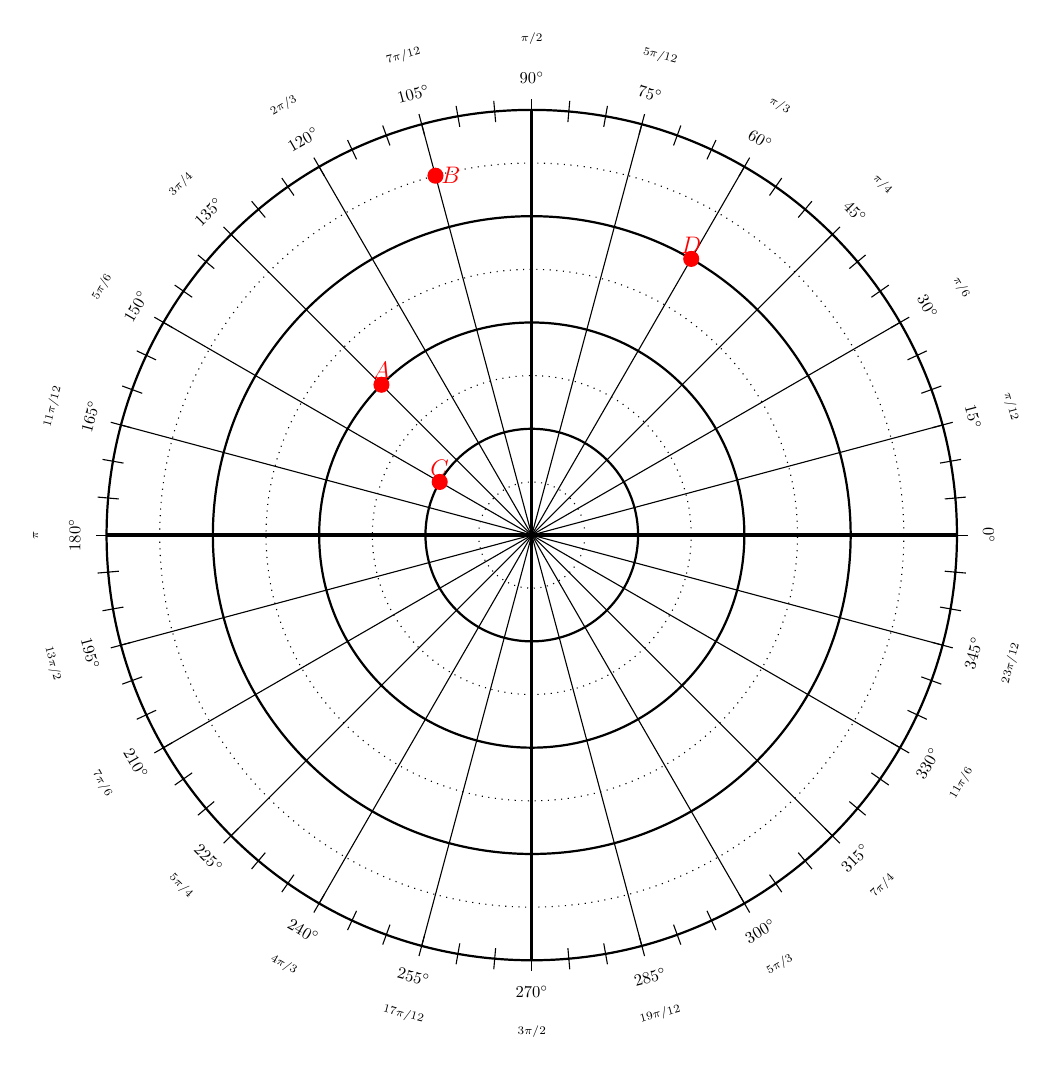
\begin{tikzpicture}[scale = 0.9, every node/.style={scale=0.6}]
    % Origin Point
    \coordinate (O) (0,0);
    % Circles
    \foreach \r in {1.5,3,...,6}
    {
        \draw[thick] (O) circle (\r cm);
    }
    
    % \foreach \r in {1.5,3,...7.5}
    % {
    %     \node at (\r, 0) [anchor=north] {\r/};
    % }
    
    \foreach \r in {0.75, 2.25,...,5.25}
    {
        \draw[dotted] (O) circle (\r cm);
    }
    
    % \node at (1.5, 0) [anchor = north west] {1};
    % \node at (3, 0) [anchor = north west] {2};
    % \node at (4.5, 0) [anchor = north west] {3};
    % \node at (6, 0) [anchor = north west] {4};
    % \node at (7.5,0) [anchor = north west] {5};
    % \foreach \r in {1.5,3,...,9}
    % {
    %     \node at (\r, 0) {\r/1.5};
    % }
    % Radial Lines
    \foreach \l in {0,15,...,360}
    {
        \draw (O) -- ++(\l:6cm);
    }
    % Thicker Radial Lines at 90 degree increments
    \foreach \l in {0,90,...,360}
    {
        \draw[very thick] (O) -- ++(\l:6cm);
    }
    % Minor Tick marks on outer circle
    \foreach \t in {0,5,...,360}
    {
        \draw (O) ++ (\t:5.85cm) -- ++(\t:0.3cm);
    }
    % Now for the fun part, the text
    % Degrees
    \node[draw=none, rotate= -90 ] at ( 0 :6.45cm) {$ 0 ^\circ$};
    \node[draw=none, rotate= -75 ] at ( 15 :6.45cm) {$ 15 ^\circ$};
    \node[draw=none, rotate= -60 ] at ( 30 :6.45cm) {$ 30 ^\circ$};
    \node[draw=none, rotate= -45 ] at ( 45 :6.45cm) {$ 45 ^\circ$};
    \node[draw=none, rotate= -30 ] at ( 60 :6.45cm) {$ 60 ^\circ$};
    \node[draw=none, rotate= -15 ] at ( 75 :6.45cm) {$ 75 ^\circ$};
    \node[draw=none, rotate= 0 ] at ( 90 :6.45cm) {$ 90 ^\circ$};
    \node[draw=none, rotate= 15 ] at ( 105 :6.45cm) {$ 105 ^\circ$};
    \node[draw=none, rotate= 30 ] at ( 120 :6.45cm) {$ 120 ^\circ$};
    \node[draw=none, rotate= 45 ] at ( 135 :6.45cm) {$ 135 ^\circ$};
    \node[draw=none, rotate= 60 ] at ( 150 :6.45cm) {$ 150 ^\circ$};
    \node[draw=none, rotate= 75 ] at ( 165 :6.45cm) {$ 165 ^\circ$};
    \node[draw=none, rotate= 90 ] at ( 180 :6.45cm) {$ 180 ^\circ$};
    \node[draw=none, rotate= 285 ] at ( 195 :6.45cm) {$ 195 ^\circ$};
    \node[draw=none, rotate= 300 ] at ( 210 :6.45cm) {$ 210 ^\circ$};
    \node[draw=none, rotate= 315 ] at ( 225 :6.45cm) {$ 225 ^\circ$};
    \node[draw=none, rotate= 330 ] at ( 240 :6.45cm) {$ 240 ^\circ$};
    \node[draw=none, rotate= 345 ] at ( 255 :6.45cm) {$ 255 ^\circ$};
    \node[draw=none, rotate= 360 ] at ( 270 :6.45cm) {$ 270 ^\circ$};
    \node[draw=none, rotate= 375 ] at ( 285 :6.45cm) {$ 285 ^\circ$};
    \node[draw=none, rotate= 390 ] at ( 300 :6.45cm) {$ 300 ^\circ$};
    \node[draw=none, rotate= 405 ] at ( 315 :6.45cm) {$ 315 ^\circ$};
    \node[draw=none, rotate= 420 ] at ( 330 :6.45cm) {$ 330 ^\circ$};
    \node[draw=none, rotate= 435 ] at ( 345 :6.45cm) {$ 345 ^\circ$};
    % Radians

    \node[draw=none, rotate= -90 ] at ( 0 :7cm) {$  $};
    \node[draw=none, rotate= -75 ] at ( 15 :7cm) {\scriptsize$ \pi/12 $};
    \node[draw=none, rotate= -60 ] at ( 30 :7cm) {\scriptsize$ \pi/6 $};
    \node[draw=none, rotate= -45 ] at ( 45 :7cm) {\scriptsize$ \pi/4 $};
    \node[draw=none, rotate= -30 ] at ( 60 :7cm) {\scriptsize$ \pi/3 $};
    \node[draw=none, rotate= -15 ] at ( 75 :7cm) {\scriptsize$ 5\pi/12 $};
    \node[draw=none, rotate= 0 ] at ( 90 :7cm) {\scriptsize$ \pi/2 $};
    \node[draw=none, rotate= 15 ] at ( 105 :7cm) {\scriptsize$ 7\pi/12 $};
    \node[draw=none, rotate= 30 ] at ( 120 :7cm) {\scriptsize$ 2\pi/3 $};
    \node[draw=none, rotate= 45 ] at ( 135 :7cm) {\scriptsize$ 3\pi/4 $};
    \node[draw=none, rotate= 60 ] at ( 150 :7cm) {\scriptsize$ 5\pi/6 $};
    \node[draw=none, rotate= 75 ] at ( 165 :7cm) {\scriptsize$ 11\pi/12 $};
    \node[draw=none, rotate= 90 ] at ( 180 :7cm) {\scriptsize$ \pi $};
    \node[draw=none, rotate= 285 ] at ( 195 :7cm) {\scriptsize$ 13\pi/2 $};
    \node[draw=none, rotate= 300 ] at ( 210 :7cm) {\scriptsize$ 7\pi/6 $};
    \node[draw=none, rotate= 315 ] at ( 225 :7cm) {\scriptsize$ 5\pi/4 $};
    \node[draw=none, rotate= 330 ] at ( 240 :7cm) {\scriptsize$ 4\pi/3 $};
    \node[draw=none, rotate= 345 ] at ( 255 :7cm) {\scriptsize$ 17\pi/12 $};
    \node[draw=none, rotate= 360 ] at ( 270 :7cm) {\scriptsize$ 3\pi/2 $};
    \node[draw=none, rotate= 375 ] at ( 285 :7cm) {\scriptsize$ 19\pi/12 $};
    \node[draw=none, rotate= 390 ] at ( 300 :7cm) {\scriptsize$ 5\pi/3 $};
    \node[draw=none, rotate= 405 ] at ( 315 :7cm) {\scriptsize$ 7\pi/4 $};
    \node[draw=none, rotate= 420 ] at ( 330 :7cm) {\scriptsize$ 11\pi/6 $};
    \node[draw=none, rotate= 435 ] at ( 345 :7cm) {\scriptsize$ 23\pi/12 $};
    \draw [color=red,fill=red] (135:3) circle (3pt) node [above] {\Large $A$};
    \draw [color=red,fill=red] (-75:-5.25) circle (3pt) node [right] {\Large $B$};
    \draw [color=red,fill=red] (-210:1.5) circle (3pt) node [above] {\Large $C$};
    \draw [color=red,fill=red] (240:-4.5) circle (3pt) node [above] {\Large $D$};
\end{tikzpicture} 
\end{minipage}
\hspace{1.5cm}
\begin{minipage}{0.3\textwidth}
\begin{enumerate}[itemsep=0.5cm]
\setcounter{enumi}{4}
    \item $\left(\frac{5\sqrt{2}}{2}, \, \frac{-5\sqrt{2}}{2}\right)$
    \item $\left(-\frac{11\sqrt{3}}{2}, \frac{11}{2}\right)$
    \item $\left(2\sqrt{3}, -2\right)$
    \item $(0, -9)$
    \item $(2, 135^\circ)$
    \item $(8, 240^\circ)$
    \item $\left(\frac{1}{2}, 330^\circ\right)$
    \item $(\sqrt{10}, 225^\circ)$
    \item $r = \frac{10}{5\cos\theta + 7\sin\theta}$
    \item $r = \frac{-1}{-2\cos\theta + \sin\theta}$
    \item $r = \frac{9}{\cos\theta - \sin\theta}$
    \item $x^{2}-4x+y^{2}=0$
    \item $x^{2}+y^{2}-2y=0$
    \item $y = 3$
    \item $x = 3$
    \item $x^2 + y^2 = 25$
    \item $y = x$
\end{enumerate}`
\end{minipage}

\end{document}


